\documentclass[varwidth=false, border=2pt]{standalone}

\usepackage{pgfplots}
\pgfplotsset{compat=1.10}
\usepackage{tikz}

\begin{document}
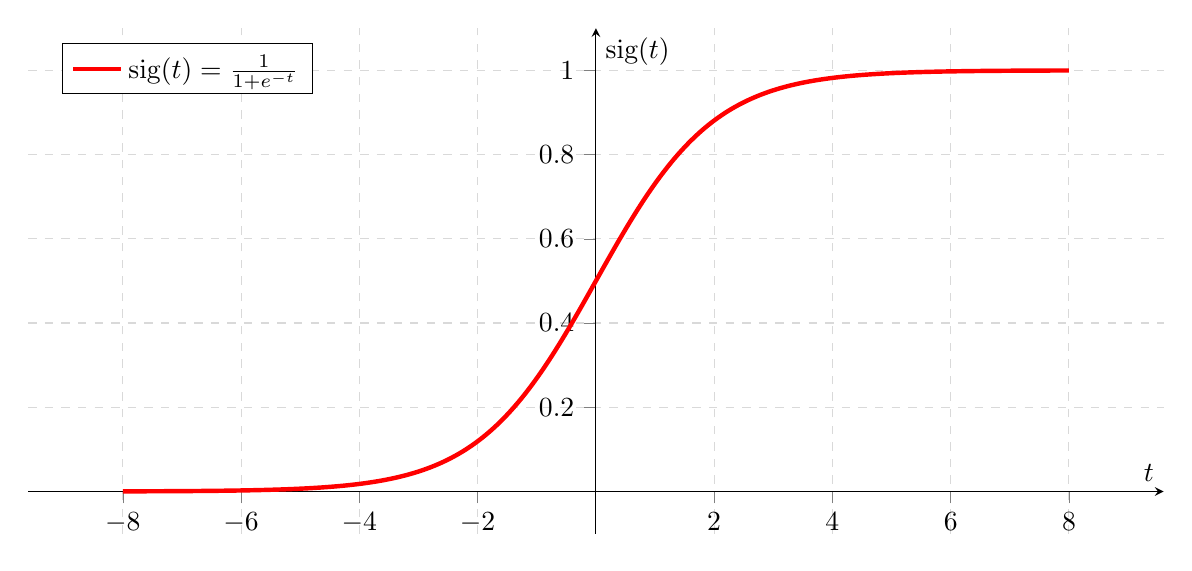
\begin{tikzpicture}
    \begin{axis}[
    	legend pos=north west,
        axis x line=middle,
        axis y line=middle,
        grid = major,
        width=16cm,
        height=8cm,
        grid style={dashed, gray!30},
        xmin=-8,     % start the diagram at this x-coordinate
        xmax= 8,    % end   the diagram at this x-coordinate
        ymin= 0,     % start the diagram at this y-coordinate
        ymax= 1,   % end   the diagram at this y-coordinate
        %axis background/.style={fill=white},
        xlabel=$t$,
        ylabel=sig$(t)$,
        tick align=outside,
        enlargelimits=true]
      % plot the stirling-formulae
      \addplot[domain=-8:8, red, ultra thick,samples=500] {1/(1+exp(-1*x))}; 
      \addlegendentry{sig$(t)=\frac{1}{1+e^{-t}}$}
    \end{axis} 
\end{tikzpicture}
\end{document}
